\documentclass[a4paper]{article}
\usepackage[utf8]{inputenc}
\usepackage[spanish, es-tabla, es-noshorthands]{babel}
\usepackage[table,xcdraw]{xcolor}
\usepackage[a4paper, footnotesep = 1cm, width=20cm, top=2.5cm, height=25cm, textwidth=18cm, textheight=25cm]{geometry}
%\geometry{showframe}

\usepackage{tikz}
\usepackage{amsmath}
\usepackage{amsfonts}
\usepackage{amssymb}
\usepackage{float}
\usepackage{graphicx}
\usepackage{caption}
\usepackage{subcaption}
\usepackage{multicol}
\usepackage{multirow}
\setlength{\doublerulesep}{\arrayrulewidth}
\usepackage{booktabs}

\usepackage{hyperref}
\hypersetup{
    colorlinks=true,
    linkcolor=blue,
    filecolor=magenta,      
    urlcolor=blue,
    citecolor=blue,    
}

\newcommand{\quotes}[1]{``#1''}
\usepackage{array}
\newcolumntype{C}[1]{>{\centering\let\newline\\\arraybackslash\hspace{0pt}}m{#1}}
\usepackage[american]{circuitikz}
\usetikzlibrary{calc}
\usepackage{fancyhdr}
\usepackage{units} 

\graphicspath{{../Ejercicio-1/}{../Ejercicio-2/}{../Ejercicio-3/}{../Ejercicio-4/}}

\pagestyle{fancy}
\fancyhf{}
\lhead{22.01 Teoría de Circuitos}
\rhead{Mechoulam, Lambertucci, Rodriguez Turco, Londero, Galdeman}
\rfoot{\centering \thepage}
\begin{document}

\subsection{Introducción}

En esta sección se implementó un filtro Band-Pass utilizando una aproximación \textbf{Chebycheff} e implementandola con celdas \textbf{Rauch}, el filtro a diseñar deberá cumplir con la siguiente plantilla.
\begin{table}[H]
\centering
\begin{tabular}{|c|c|}
\hline
$Pendiente$      & -40$\frac{dB}{dec}$           \\ \hline
$f_p$      & 28kHz          \\ \hline
$B$      & $\frac{1}{10}$           \\ \hline
$A_p$      & 3dB               \\ \hline
$Filtro$      & BP              \\ \hline
$|Z_{in}|$ & $\geq 50k \Omega$ \\ \hline
\end{tabular}
\end{table}
\subsection{Aproximación de Chebycheff.}
Para esta sección se utlizó la aproximación de \textbf{Chebyfeff}, además se propuso una plantilla mas restrictiva, con el fin de asegurar el cumplimiento de la original. 

Se despejó el valor de $f_p^+$ y $f_p^-$ 
\begin{align}
f_0^2 = f_p^+ \cdot f_p^- \\
B = \frac{\Delta f_p}{f_0}\\
f_p^+ =29.435 kHz  \ \ \ f_p^- = 26.635 kHz
\end{align}
Luego teniendo en cuenta que la pendiente originalmente es de 40dB por decada se tomo la frecuencia de atenuación acorde  talque mantenga las condiciones de simetría, siendo estas: $f_a^+= 294.35kHz y f_a^- = 2.635kHz$.


Siendo esta la plantilla final.
\begin{table}[H]
\centering
\begin{tabular}{|c|c|}
\hline
$f_s^-$      & 2.6635 kHz          \\ \hline
$f_p^-$      & 26.635 kHz         \\ \hline
$f_p^+$      & 29.435 kHz           \\ \hline
$f_s^+$      & 294.35 kHz          \\ \hline
$A_s$      & 40dB           \\ \hline
$A_p$      & 1dB               \\ \hline
\end{tabular}
\end{table}
Obteniendo la siguiente función transferencia:
\begin{align}
	H(s)=\frac{s}{\left( \frac{s}{23728.54}\right) ^2+s\cdot \frac{23728.54}{3.23}+1}\cdot \frac{s}{\left( \frac{s}{33052.25} \right)^2+s\cdot \frac{33052.25}{3.23}+1}
\end{align}
al cual le corresponde la siguiente respues en frecuencia:

Y el siguiente diagrama de polos y ceros:
\begin{figure}[H]
	\centering
	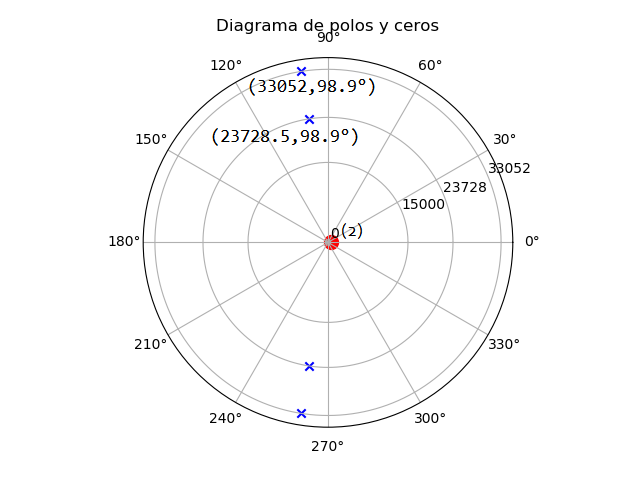
\includegraphics[width=0.5\textwidth]{Imagenes-Ej2/DiagramaPolosYCeros.png}
	\label{fig:stepresponse}
	\caption{Diagrama Polos y Ceros}
\end{figure}

Teniendo los pares de polos conjugados un Q de 3.23	


\subsubsection{Elecciones de diseño}
Se decidió armar etapas con celdas segundo orden en cascada dado a que el orden es 4.
Para la asociación de polos se tomo criterio agrupar cada par de polos con 1 cero , agrupandolos de las siguiente forma.
\begin{figure}[H]
	\centering
	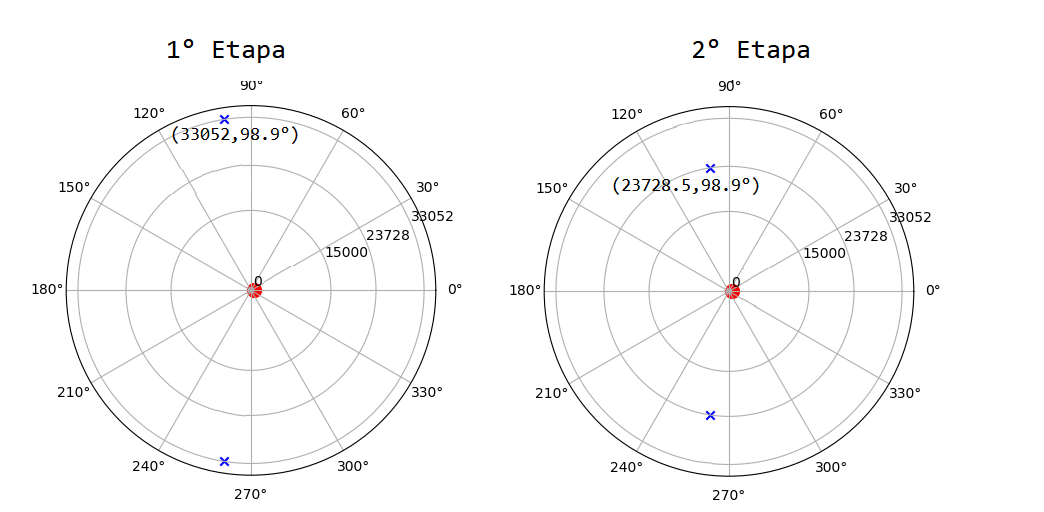
\includegraphics[width=\textwidth]{Imagenes-Ej2/UnionCeros.png}
	\label{fig:CeroPoleUnion}
	\caption{Diagrama Polos y Ceros para cada etapa}
\end{figure}

\subsection{Celda Rauch.}
La celda Rauch es una modificación de la celda Deliyannis-Friend incluyendo uan realimentación positiva.
\begin{figure}[H]
	\centering
	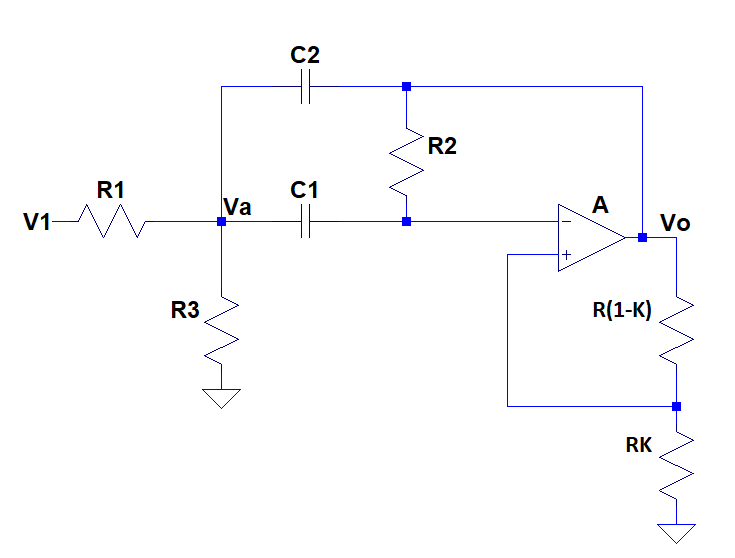
\includegraphics[width=0.5\textwidth]{Imagenes-Ej2/Circuit.PNG}
	\label{fig:graph}
	\caption{Circuito celda Rauch Band-Pass.}
\end{figure}
\subsubsection{Cálculo Analítico}
---
\subsubsection{Elecciones de diseño}

\begin{center}
	\huge{\textcolor{red}{\textbf{Tabla sensibilidades}}}
\end{center}
En base a esta tabla se tomo especial cuidado en la elección de componentes y en el matcheo de impedancias.

Los componentes utilizados fueron los siguientes:
\begin{table}[H]
\centering
\begin{tabular}{lllll}
\multicolumn{1}{c}{Componente} & \multicolumn{1}{c}{1er Etapa} & \multicolumn{1}{c}{Composición} & 2da Etapa      & Composición           \\ \hline
$R_1$                          & $7.3 k\Omega$                 & $10k // 27k  \Omega$            & $5.24 k\Omega$ & $5.6k // 82k  \Omega$ \\
$R_2$                          & $5.56 k\Omega$                & $5.6k // 680k  \Omega$          & $3.99 k\Omega$ & $82 + 3.9k  \Omega$   \\
$R_3$                          & $1.43 k\Omega$                & $1.5 k // 33k  \Omega$          & $1.03k\Omega$  & $27 + 1k  \Omega$     \\
$R_4$                          & $3.49 k\Omega$                & $3.9k // 33k  \Omega$           & $3.49 k\Omega$ & $3.9k // 33k  \Omega$ \\
$R_5$                          & $1 k\Omega$                   & $1 k  \Omega$                   & $1 k\Omega$    & $1 k\Omega$           \\
$C_1$                          & 2.2 nF                        & 2.2 nF                          & 2.2 nF         & 2.2 nF                \\
$C_2$                          & 2.2 nF                        & 2.2 nF                          & 2.2 nF         & 2.2 nF               
\end{tabular}
\end{table}

Se calculó el error porcentual asociado a la aproximación de la resistencias viendose en la siguiente tabla.
\begin{table}[H]
\centering
\begin{tabular}{lll}
\multicolumn{1}{c}{Error Porcentual} & \multicolumn{1}{c}{1er Etapa} & \multicolumn{1}{c}{2da Etapa} \\ \hline
$R_1$                                & 0.1 $\%$                      & $0.038  \%$                   \\
$R_2$                                & 0.1 $\%$                      & 0.2 $\%$                      \\
$R_3$                                & 0.4 $\%$                      & 0.1 $\%$                      \\
$R_4$                                & 0.1 $\%$                      & 0.1 $\%$                      \\
$R_5$                                & $\approx 0 \%$                & $\approx 0 \%$                \\
$C_1$                                & $\approx 0 \%$                & $\approx 0 \%$                \\
$C_1$                                & $\approx 0 \%$                & $\approx 0 \%$               
\end{tabular}
\end{table}

Cabe destacar que todas las imepdancias que fueron colocadas en el circuito fueron elegidas entre varias de su mismo tipo, con la finalidad de poner impedancias que sean realmente de los valores deseados.

\subsubsection{Acoplamiento de Impedancias.}

Para que ambas etapas no se carguen entre si la impedancia de entrada de la segunda etapa debe ser mucho mayor a la de salida de la primera, para lo siguiente se obtuvieron las impedancias de entrada de ambas celdas, incluyendo la de salida de la primera.
\begin{figure}[H]
	\centering
	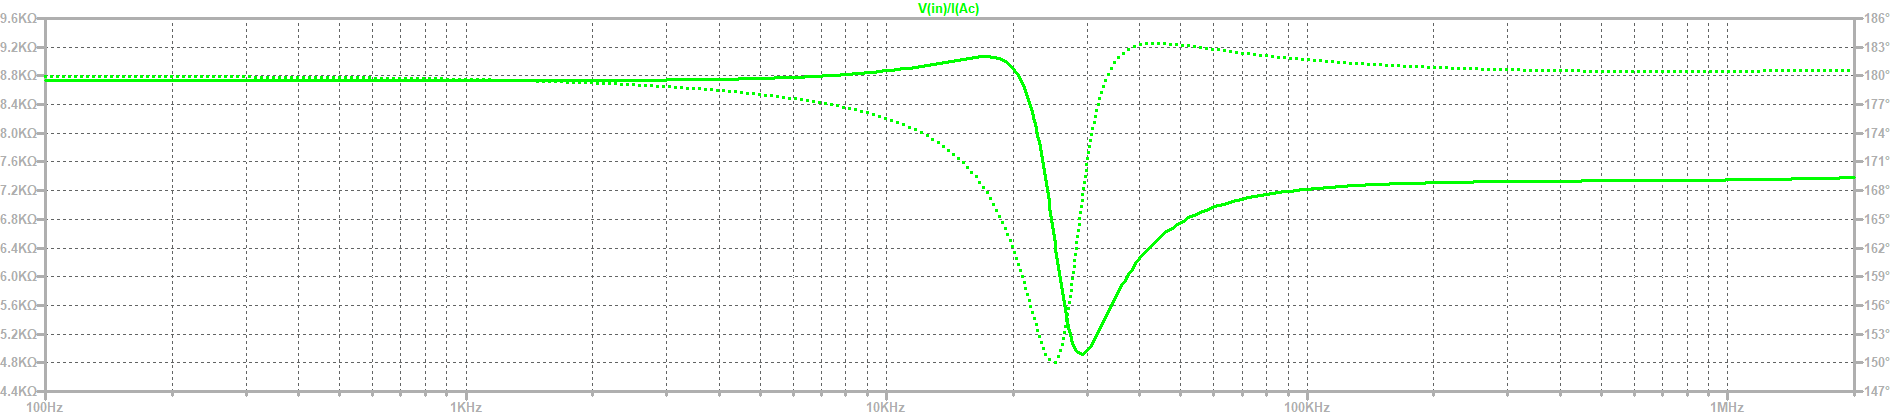
\includegraphics[width=\textwidth]{Imagenes-Ej2/ZinE1.png}
	\label{fig:graph}
	\caption{Impedancia de entrada 1er etapa.}
\end{figure}

\begin{figure}[H]
	\centering
	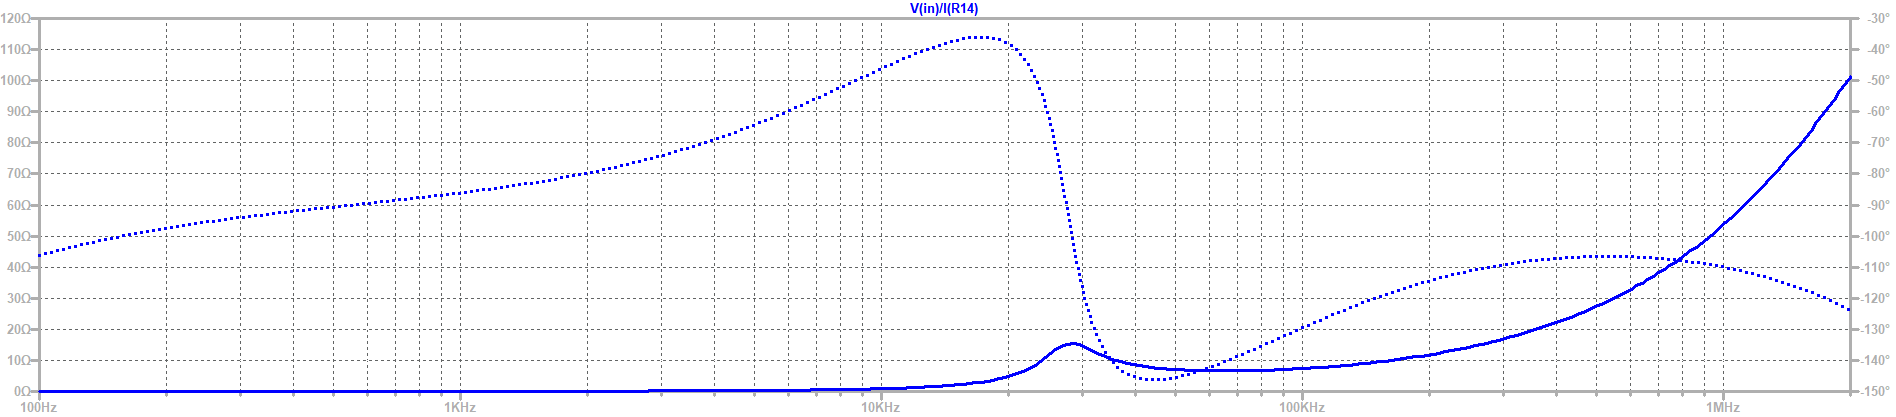
\includegraphics[width=\textwidth]{Imagenes-Ej2/ZoutE1.png}
	\label{fig:graph}
	\caption{Impedancia de salida 1er etapa.}
\end{figure}


\begin{figure}[H]
	\centering
	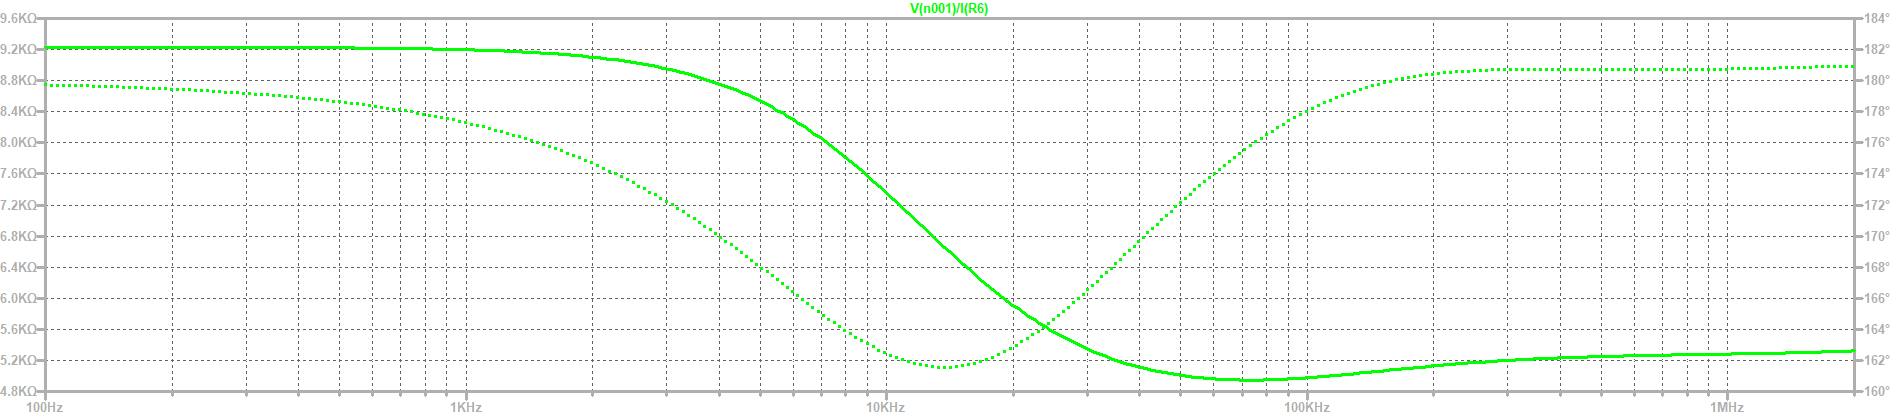
\includegraphics[width=\textwidth]{Imagenes-Ej2/ZinE2.png}
	\label{fig:graph}
	\caption{Impedancia de entrada 2da etapa.}
\end{figure}

\subsection{Respuesta en Frecuencia.}
Se realizó un análisis de Montecarlo a la respuesta en frecuencia del circuito, utilizando una tolerancia de las resistencias al 1$\%$ y capacitores al 10$\%$ obteniendo la siguiente disperción.
%\begin{figure}[H]
%	\centering
%	\includegraphics[width=0.4\textwidth]{/ImagenesEjercicio3/Graph.png}
%	\label{fig:graph}
%\end{figure}
También se midió la respuesta en frecuencia del filtro y se cotejó con la simulación.
\begin{figure}[H]
	\centering
	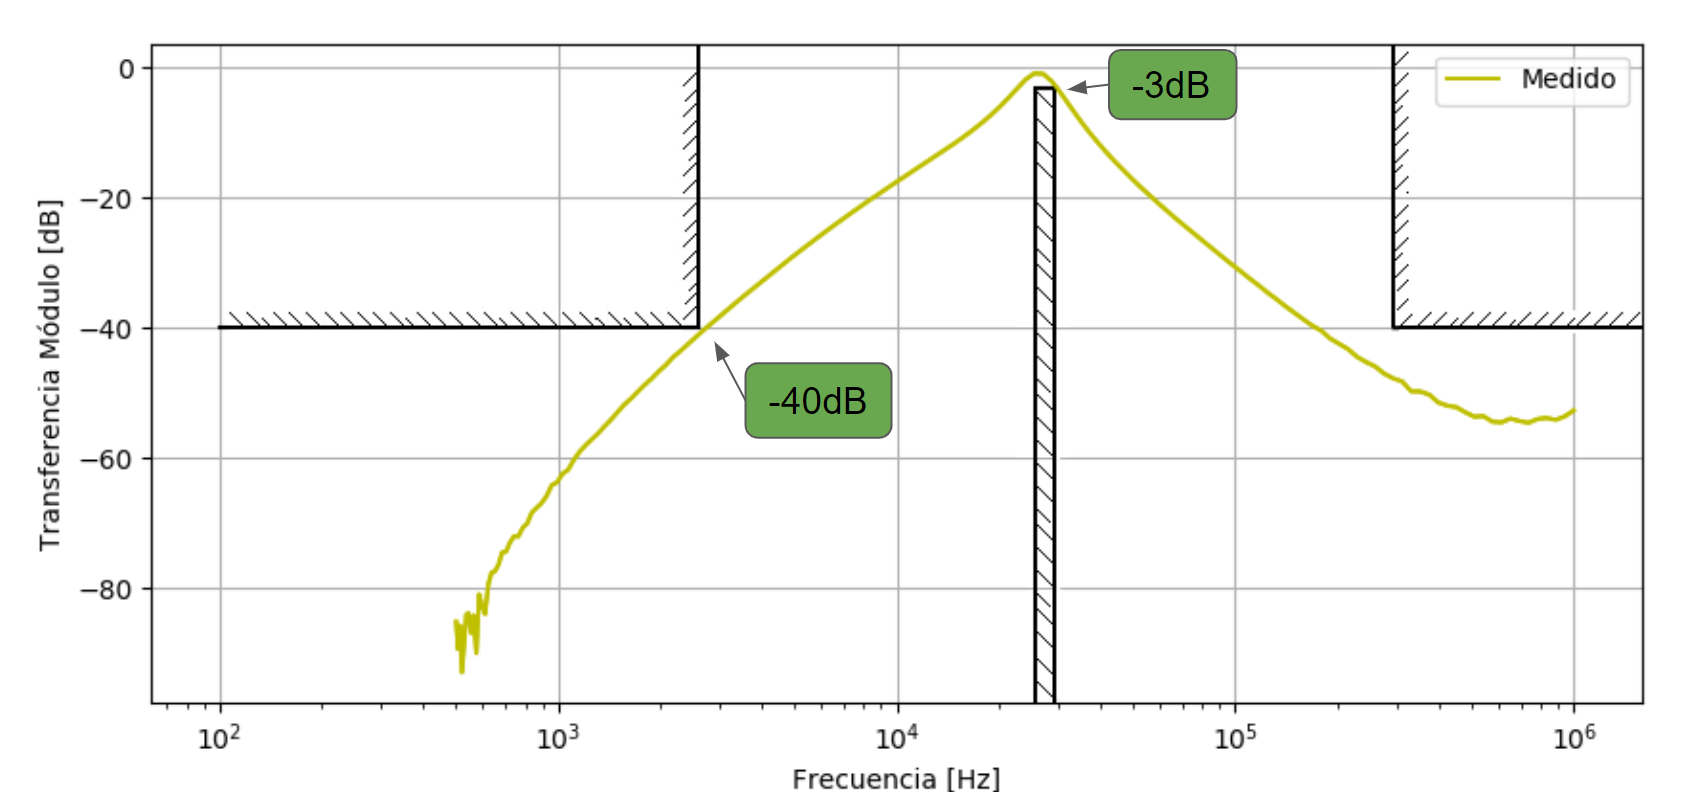
\includegraphics[width=\textwidth]{Imagenes-Ej2/BodeRauch.png}
	\label{fig:graph}
\end{figure}
\begin{figure}[H]
	\centering
	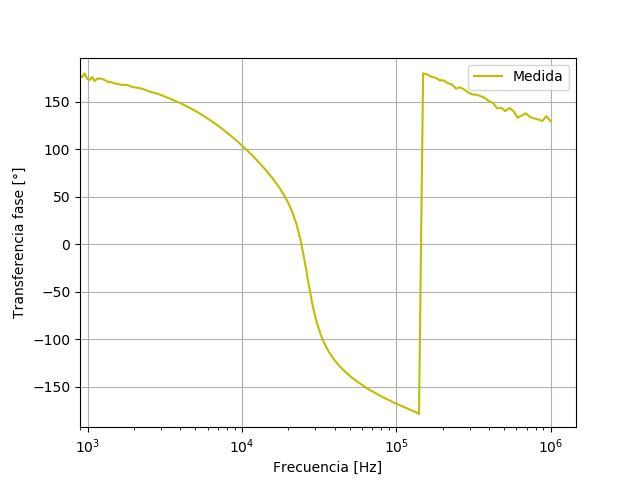
\includegraphics[width=\textwidth]{Imagenes-Ej2/BodeRauchFase.png}
	\label{fig:graph}
\end{figure}

\subsubsection{Etapas.}
Se realizaron 2 etapas, ambas siendo el mismo tipo de celda, pero con distintos parámetros.
\subsubsection{Filtro definitivo.}
%
%\begin{figure}[H]
%	\centering
%	\includegraphics[width=0.4\textwidth]{/ImagenesEjercicio3/Graph.png}
%	\label{fig:graph}
%\end{figure}

\end{document}